\setlength{\footskip}{8mm}

\chapter{EXPERIMENT}

Based on \ref{metho-s1} and \ref{metho-s2}, To remove undesirable spectral data from acquired spectra, we first measure the background noises (e.g., sample slide, air) as the starting spectral value from the Raman instrument as shown in Figure 4.1.
\\
Second, we collected blood sample from index finger in fasting condition of 5 to 6 hours for 6 times on sample slide. From the above mentioned, in Figure 4.2 we can see the sample slide peak obviously because of difficulty of uncontrollably blood shedding on it. To eliminate mistakes from this peak in future experiments, we must carefully manage how blood is placed on the sample slide and keep it centered on one location.
\\
We normalized the sample spectra with the lipid peak (1450 $cm-1$) and the hemoglobin peak (1549 $cm-1$, as illustrated in Figures 4.3 and 4.4. Although the preprocessing experiment did not go as expected, and the blood sample did not show a glucose peak (1125 $cm-1$) obviously, it will be fully developed in future study.

\begin{figure}
    \caption{Raman spectra background noises.}
    \centerline{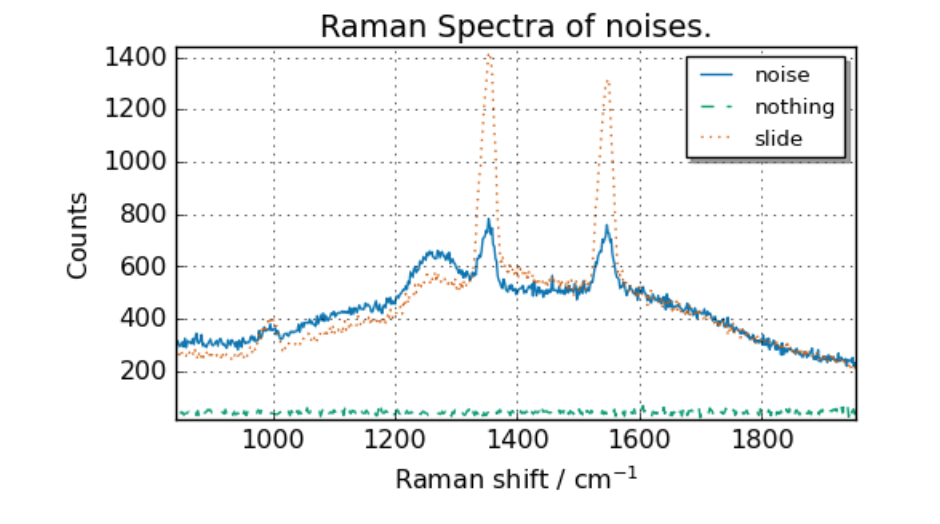
\includegraphics[width=3in]{figures/background-noise.png}} \label{fig:bgnoise}
    % \small{\textit{Note.} Additional notes goes here.}
\end{figure}


\begin{figure}
    \caption{Raman spectra of blood sample from index finger.}
    \centerline{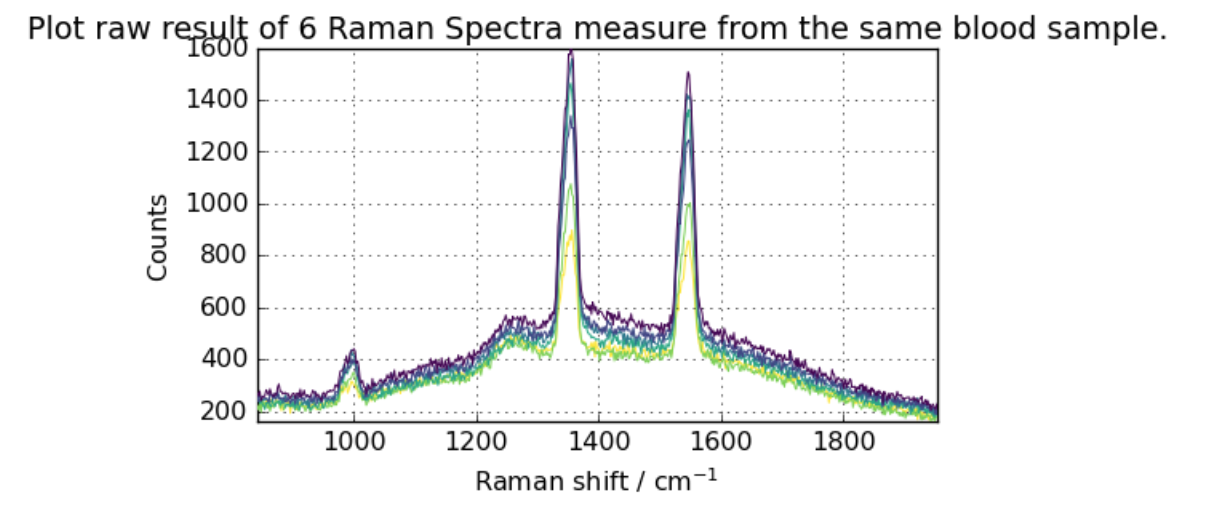
\includegraphics[width=3in]{figures/bloodsample.png}} \label{fig:bloodsample}
    % \small{\textit{Note.} Additional notes goes here.}
\end{figure}

\begin{figure}
    \caption{Raman spectra of blood sample with lipid normalized.}
    \centerline{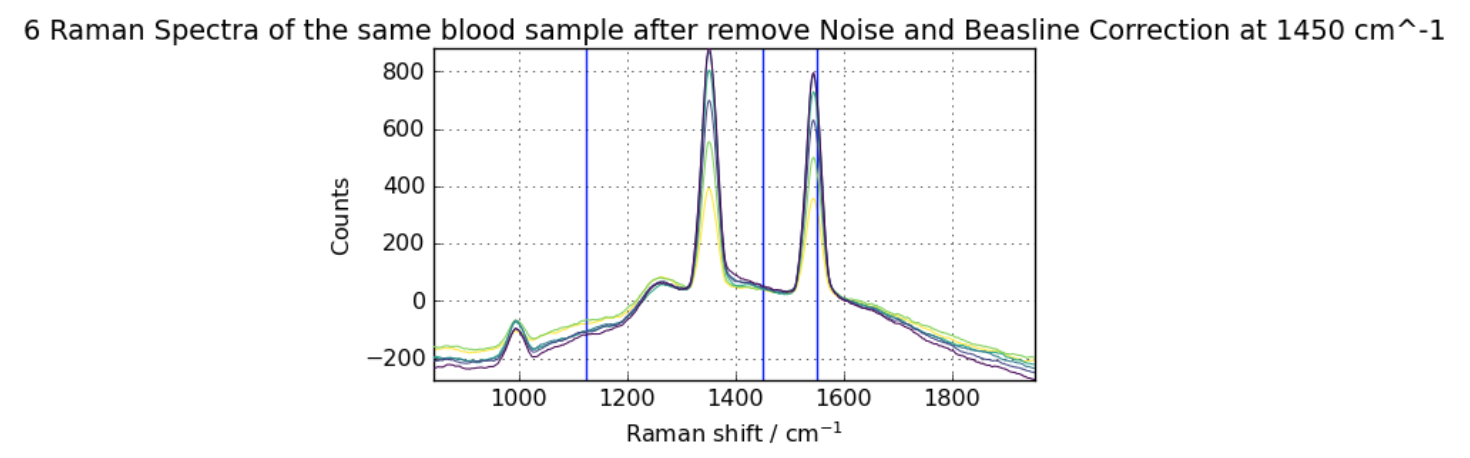
\includegraphics[width=3in]{figures/normalized-lipid-peak.png}} \label{fig:lipidnorm}
    % \small{\textit{Note.} Additional notes goes here.}
\end{figure}

\begin{figure}
    \caption{Raman spectra of blood sample with hemoglobin normalized.}
    \centerline{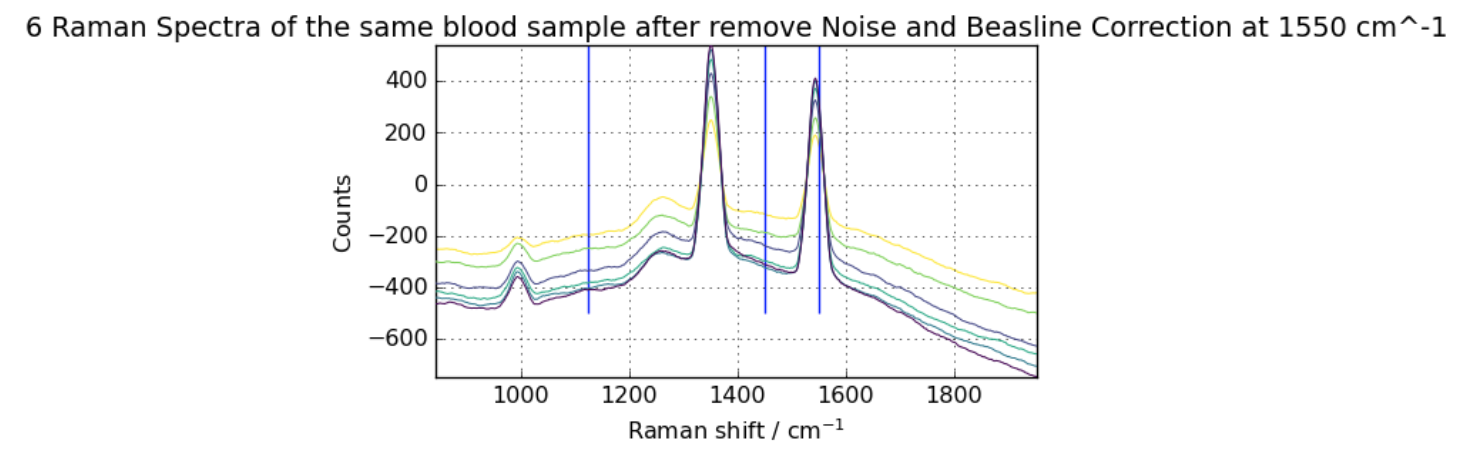
\includegraphics[width=3in]{figures/normalized-hemoglobin-peak.png}} \label{fig:hemoglobinnorm}
    % \small{\textit{Note.} Additional notes goes here.}
\end{figure}

